\documentclass[10pt,twocolumn,letterpaper]{article}
\usepackage{cvpr}

\usepackage{graphicx}
\usepackage{amsmath}
\usepackage{amssymb}
\usepackage{booktabs}
\usepackage{multirow}
\usepackage{colortbl}
\usepackage{xcolor}
\usepackage{enumitem}

\definecolor{cvprblue}{rgb}{0.21,0.49,0.74}
\usepackage[pagebackref,breaklinks,colorlinks,allcolors=cvprblue]{hyperref}

\definecolor{bestcolor}{RGB}{144,238,144}
\definecolor{secondcolor}{RGB}{173,216,230}
\newcommand{\best}[1]{\cellcolor{bestcolor}\textbf{#1}}
\newcommand{\second}[1]{\cellcolor{secondcolor}#1}

\def\paperID{33025}
\def\confName{CVPR}
\def\confYear{2026}

\begin{document}

\title{CRYSTAL: Updated GRPO Results and Reviewer Responses}

\maketitle
\thispagestyle{empty}

%%%%%%%%%%%%%%%%%%%%%%%%%%%%%%%%%%%%%%%%%%%%%%%%%%%%%%%%%%%%%%%%%%%%%%%%%%%%
\section{Addressing the Central GRPO Concern}
\label{sec:central}
%%%%%%%%%%%%%%%%%%%%%%%%%%%%%%%%%%%%%%%%%%%%%%%%%%%%%%%%%%%%%%%%%%%%%%%%%%%%

The meta-review and all three reviewers identified the GRPO experiments as the weakest part of the submission: training with step-level rewards \textit{decreased} Match-F1 (0.480$\to$0.426), undermining the claim that CRYSTAL can guide model improvement. We address this with \textbf{two new experiments} that isolate the source of the problem and demonstrate that Match-F1 \textit{can} serve as an effective training signal when the reward structure is properly designed. (All Match-F1 scores use the ablation-validated \texttt{all-distilroberta-v1} encoder, $\tau$=0.35.)

Table~\ref{tab:headline} presents the headline comparison.

\begin{table}[t]
\centering
\caption{\textbf{Three GRPO strategies compared.} All train Qwen2.5-VL-3B on 4$\times$A100 with DeepSpeed ZeRO-3. $\Delta$F1 relative to baseline (0.480).}
\label{tab:headline}
\resizebox{\columnwidth}{!}{
\begin{tabular}{lccccl}
\toprule
\textbf{Strategy} & \textbf{Acc (\%)} & \textbf{M-F1} & \textbf{$\Delta$F1} & \textbf{Rec} & \textbf{Collapse?} \\
\midrule
Baseline          & 39.85 & 0.480 & --       & 0.347 & -- \\
\midrule
Composite (paper) & \best{44.92} & 0.426 & $-$11\%  & 0.284 & Yes (step 600) \\
Answer-Only       & 44.90 & 0.433 & $-$10\%  & 0.313 & No \\
\textbf{CPR}      & 41.38 & \best{0.633} & \best{+32\%} & \best{0.488} & No \\
\bottomrule
\end{tabular}
}
\end{table}

\noindent\textbf{Why the original composite training failed.} Answer-Only (format~+~accuracy, \textit{no reasoning reward}) reaches the same accuracy as Composite (44.90 vs 44.92\%), proving the accuracy reward alone drives that improvement. In Composite, the additive reward structure lets accuracy dominate: the model learns to maximize precision (0.983) by generating fewer steps (3.00 avg), collapsing recall to 0.284. The Match-F1 decrease is not a flaw in the metric, but a consequence of accuracy reward domination in an unbalanced composite.

\noindent\textbf{CPR resolves this conflict.} The Causal Process Reward uses a multiplicative interaction that \textit{requires} both correct answers and aligned reasoning:
\begin{equation}
R_{\text{CPR}} = \begin{cases}
0.6 + 0.4 \cdot \text{F1}_{\text{step}} & \text{if correct} \\
0.4 \cdot \text{F1}_{\text{step}} \cdot 0.3 & \text{if wrong}
\end{cases}
\end{equation}
Combined with PCGrad~\cite{yu2020pcgrad} for gradient conflict resolution, CPR achieves Match-F1~=~0.633 (+32\% over baseline) while improving accuracy to 41.38\%.

Figure~\ref{fig:summary_bars} provides a visual summary. Composite achieves the highest accuracy but the lowest reasoning quality. Answer-Only matches that accuracy without improving reasoning. CPR sacrifices 3.5pp accuracy to gain +32\% in reasoning quality, achieving the most balanced outcome.

\begin{figure}[t]
\centering
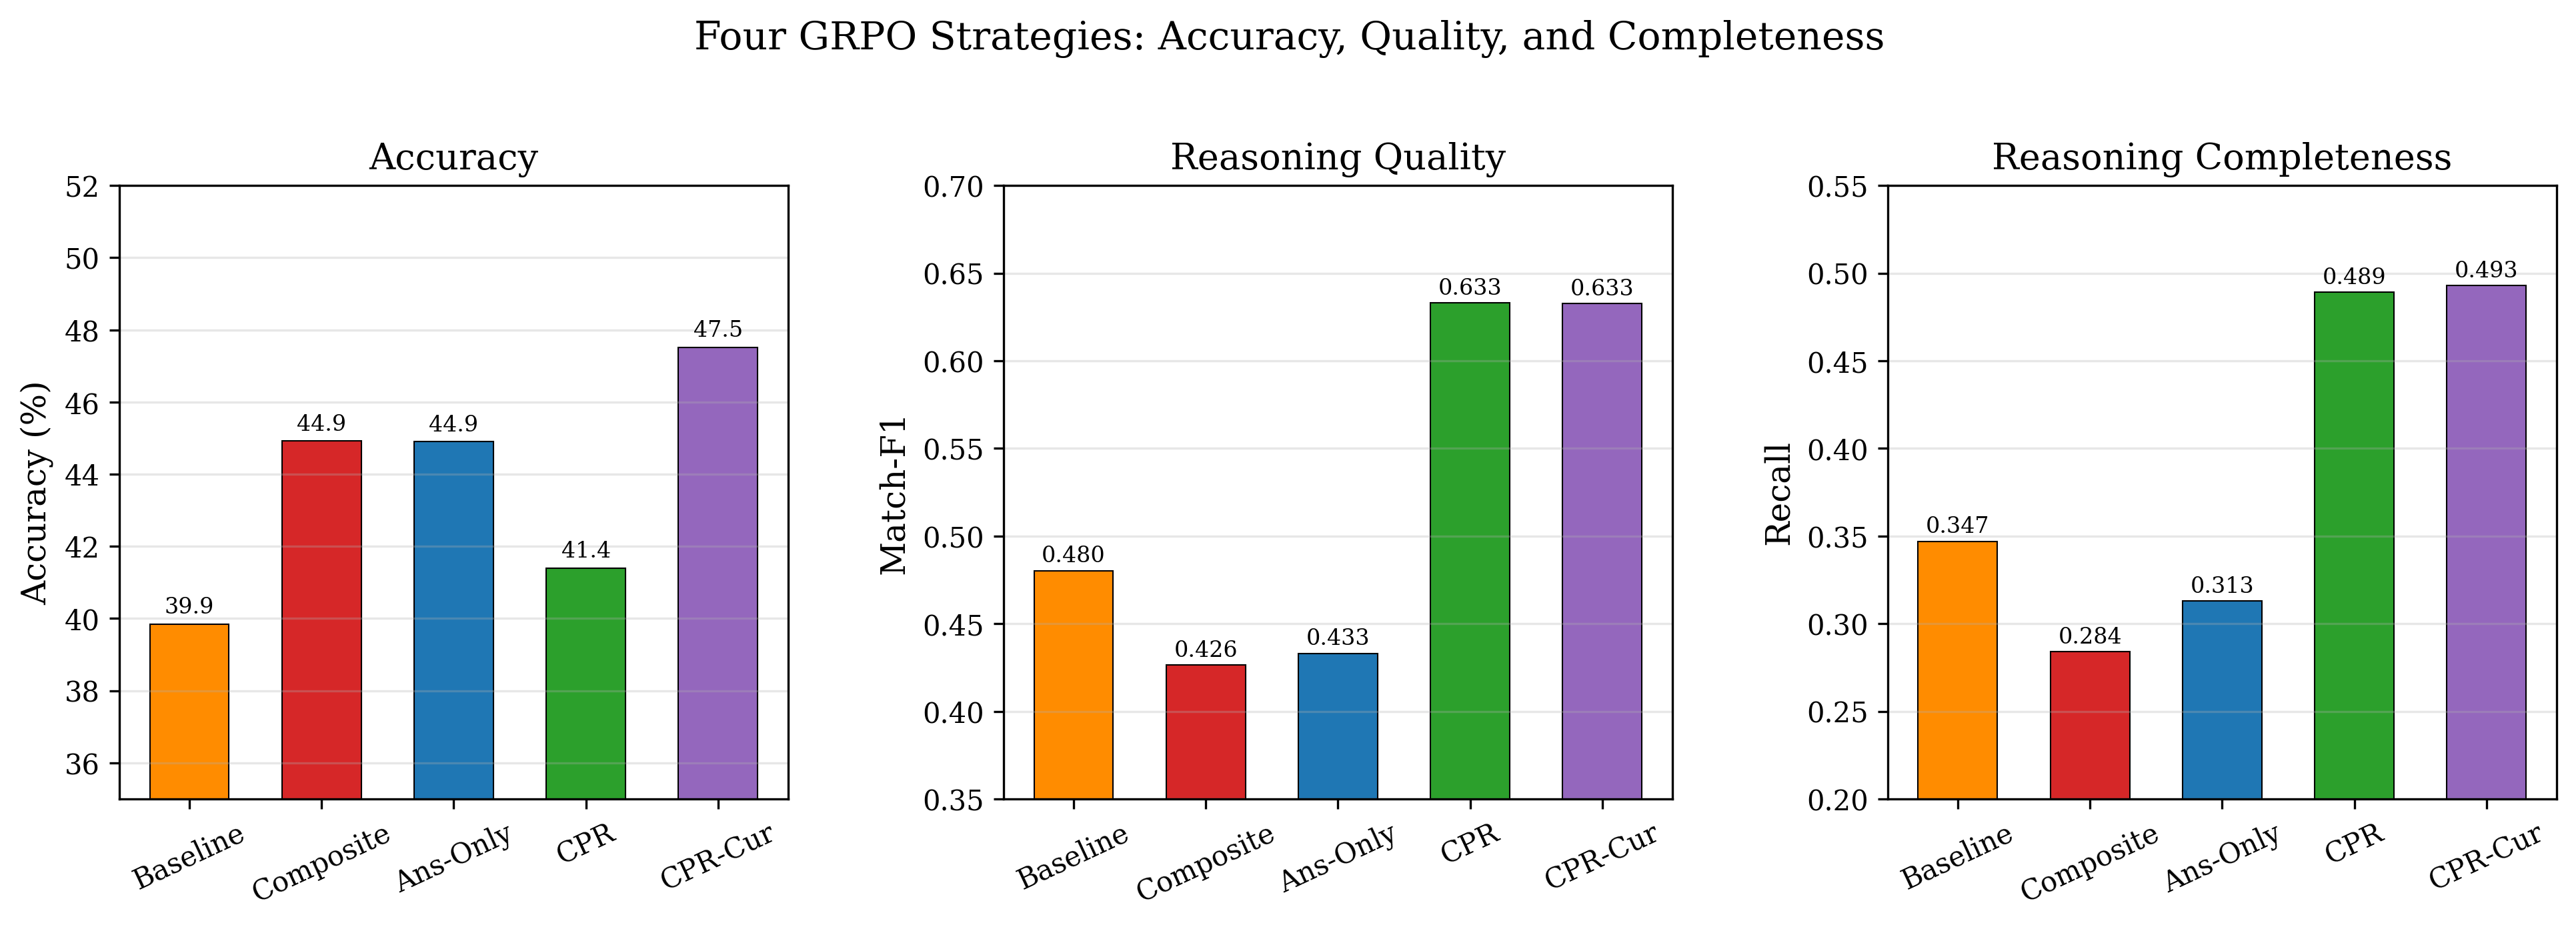
\includegraphics[width=\columnwidth]{figures/grpo_summary_bars.png}
\caption{\textbf{Side-by-side comparison of three strategies} on accuracy, Match-F1, and recall. CPR is the only strategy that improves Match-F1 (+32\%) and recall (+41\%) above baseline while maintaining competitive accuracy.}
\label{fig:summary_bars}
\end{figure}

%%%%%%%%%%%%%%%%%%%%%%%%%%%%%%%%%%%%%%%%%%%%%%%%%%%%%%%%%%%%%%%%%%%%%%%%%%%%
\section{Full Training Trajectories}
\label{sec:trajectories}
%%%%%%%%%%%%%%%%%%%%%%%%%%%%%%%%%%%%%%%%%%%%%%%%%%%%%%%%%%%%%%%%%%%%%%%%%%%%

\subsection{Composite GRPO (Original Paper)}

Reward: $2.0 \cdot R_{\text{fmt}} + 2.0 \cdot R_{\text{acc}} + 2.0 \cdot R_{\text{reasoning}}$ (word-overlap).

\begin{table}[t]
\centering
\caption{\textbf{Composite GRPO trajectory.} Hard mode collapse at step 600.}
\label{tab:composite}
\resizebox{\columnwidth}{!}{
\begin{tabular}{rcccccl}
\toprule
\textbf{Step} & \textbf{Acc} & \textbf{F1} & \textbf{Prec} & \textbf{Rec} & \textbf{Steps} & \textbf{Phase} \\
\midrule
0     & 39.85 & 0.480 & 0.898 & 0.347 & 3.73 & Baseline \\
100   & 30.30 & 0.177 & 0.997 & 0.101 & 1.00 & Warm-up \\
200   & 35.66 & 0.365 & 0.930 & 0.238 & 2.49 & Warm-up \\
300   & 28.91 & \best{0.507} & 0.967 & \best{0.359} & 3.77 & Peak F1 \\
400   & 30.41 & 0.329 & 0.993 & 0.204 & 2.09 & Collapsing \\
500   & 30.30 & 0.388 & 0.987 & 0.250 & 2.63 & Collapsing \\
600   & 26.98 & 0.305 & 0.927 & 0.189 & 1.93 & \textbf{Hard collapse} \\
700   & 38.92 & 0.506 & 0.952 & 0.359 & 3.82 & Partial recovery \\
800   & 36.17 & 0.468 & 0.878 & 0.341 & 3.72 & Unstable \\
900   & 39.83 & 0.473 & 0.949 & 0.330 & 3.55 & Recovering \\
1000  & 42.04 & 0.383 & 0.965 & 0.248 & 2.62 & Acc dominates \\
1100  & 39.66 & 0.502 & 0.972 & 0.353 & 3.76 & Oscillation \\
1200  & 37.04 & 0.480 & 0.944 & 0.335 & 3.55 & Oscillation \\
1300  & 35.00 & 0.377 & 0.970 & 0.243 & 2.53 & Oscillation \\
1400  & \best{44.92} & 0.426 & \best{0.983} & 0.284 & 3.00 & Best acc \\
1500  & 44.79 & 0.410 & 0.975 & 0.270 & 2.85 & Plateau \\
\bottomrule
\end{tabular}
}
\end{table}

\subsection{Answer-Only GRPO (New Experiment)}

Reward: $2.0 \cdot R_{\text{fmt}} + 2.0 \cdot R_{\text{acc}}$ with \textit{no reasoning component}. This experiment was requested by Reviewer Aho6 to isolate the effect of step-level supervision.

\begin{table}[t]
\centering
\caption{\textbf{Answer-Only trajectory.} Stable, no collapse. Match-F1 remains flat (0.41 to 0.44) throughout training. Reasoning does not improve without reasoning reward.}
\label{tab:answeronly}
\resizebox{\columnwidth}{!}{
\begin{tabular}{rcccccl}
\toprule
\textbf{Step} & \textbf{Acc} & \textbf{F1} & \textbf{Prec} & \textbf{Rec} & \textbf{Steps} & \textbf{Phase} \\
\midrule
0     & 39.85 & 0.480 & 0.898 & 0.347 & 3.73 & Baseline \\
150   & 37.99 & 0.406 & 0.731 & 0.295 & 3.64 & Early \\
300   & 42.56 & 0.411 & 0.753 & 0.297 & 3.62 & Improving \\
600   & 44.07 & \best{0.436} & 0.790 & \best{0.316} & 4.00 & Strong acc \\
1400  & \best{44.90} & 0.433 & \best{0.802} & 0.313 & 3.85 & Best acc \\
1500  & 44.30 & 0.429 & 0.803 & 0.308 & 3.78 & Plateau \\
\bottomrule
\end{tabular}
}
\end{table}

\subsection{Causal Process Reward (New Experiment)}

Reward: $2.0 \cdot R_{\text{fmt}} + 2.0 \cdot R_{\text{acc}} + 2.0 \cdot R_{\text{causal}}$ with PCGrad.

\begin{table}[t]
\centering
\caption{\textbf{CPR trajectory.} Soft collapse at step 700 with full self-correction. Both accuracy and F1 improve simultaneously from step 700 to 2400.}
\label{tab:cpr}
\resizebox{\columnwidth}{!}{
\begin{tabular}{rcccccl}
\toprule
\textbf{Step} & \textbf{Acc} & \textbf{F1} & \textbf{Prec} & \textbf{Rec} & \textbf{Steps} & \textbf{Phase} \\
\midrule
0     & 39.85 & 0.480 & 0.898 & 0.347 & 3.73 & Baseline \\
400   & 39.96 & 0.704 & 0.988 & 0.571 & 6.00 & Rapid F1 gain \\
500   & 36.30 & \best{0.714} & 0.972 & \best{0.590} & 6.23 & Peak F1 \\
700   & 38.31 & 0.433 & 0.792 & 0.309 & 3.15 & Soft collapse \\
1000  & 37.71 & 0.600 & 0.988 & 0.448 & 4.71 & Recovery \\
1400  & 40.07 & 0.556 & 0.982 & 0.402 & 4.19 & Stabilizing \\
2000  & 40.33 & 0.565 & 0.970 & 0.416 & 4.32 & Sustained gain \\
\best{2400} & \best{41.38} & 0.633 & \best{0.975} & 0.488 & 5.11 & \best{Best} \\
\bottomrule
\end{tabular}
}
\end{table}

\subsection{Training Dynamics Visualization}

Figure~\ref{fig:f1_traj} overlays the Match-F1 trajectories for all three strategies. The Composite curve (red) oscillates wildly between 0.18 and 0.51 due to the accuracy-reasoning conflict. Answer-Only (blue) stays nearly flat, confirming that removing the reasoning signal removes any F1 variation. CPR (green) shows a clear V-shape: an initial dip at step 700 followed by monotonic recovery through step 2400, reaching the highest F1 of any strategy.

\begin{figure}[t]
\centering
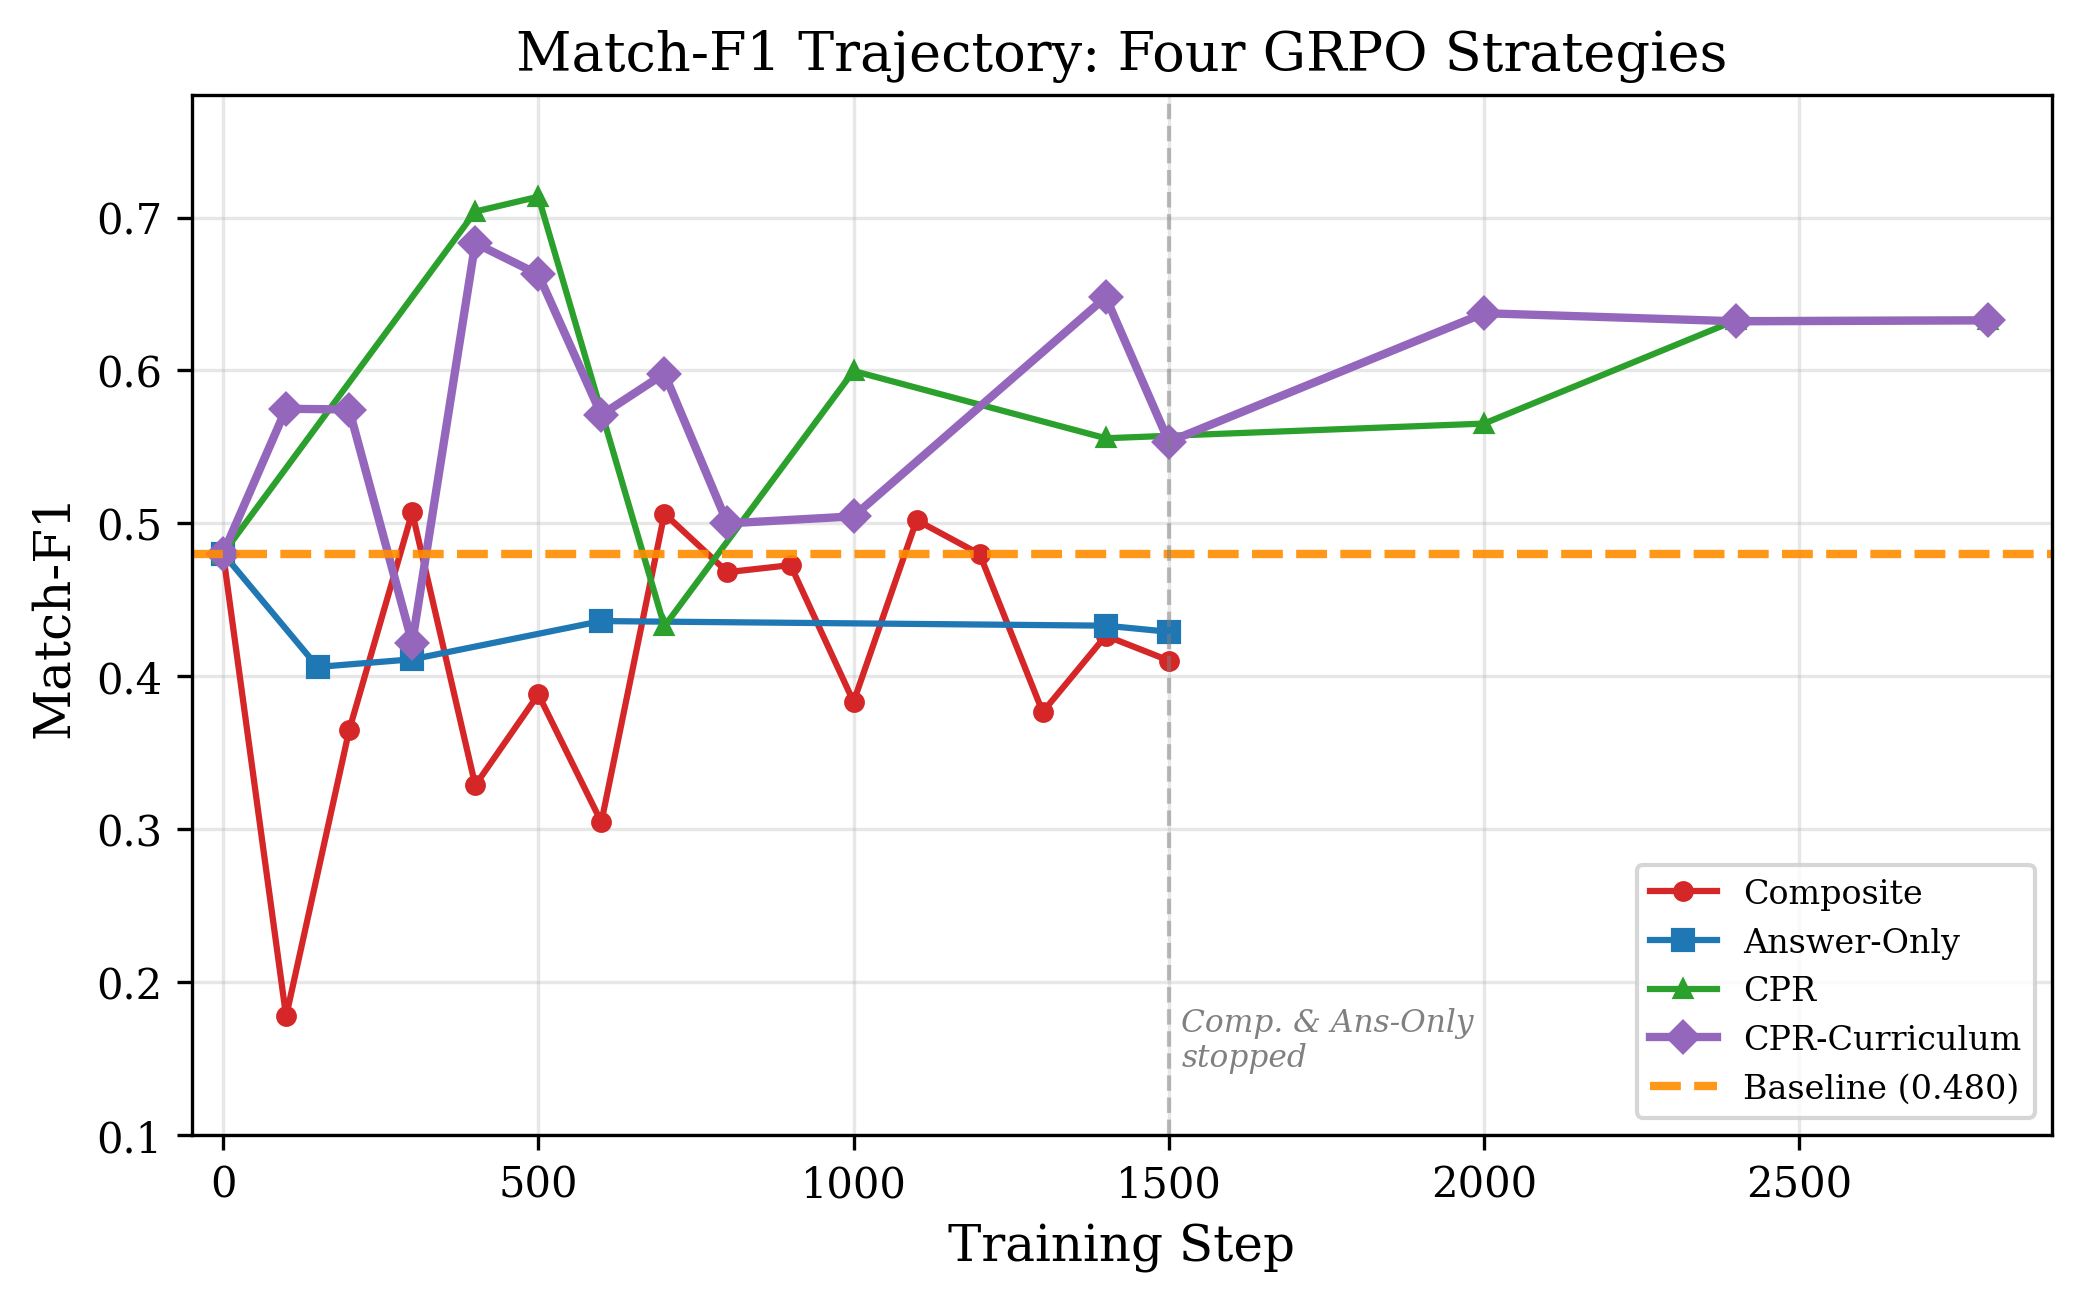
\includegraphics[width=\columnwidth]{figures/grpo_f1_trajectory.png}
\caption{\textbf{Match-F1 training trajectories.} Composite oscillates due to accuracy-reasoning gradient conflict. Answer-Only remains flat (no reasoning reward). CPR recovers from soft collapse and improves monotonically from step 700 to 2400.}
\label{fig:f1_traj}
\end{figure}

Figure~\ref{fig:acc_traj} reveals \textbf{why accuracy alone is an insufficient training metric}. Answer-Only achieves the highest and most stable accuracy (44.90\%), yet Figure~\ref{fig:f1_traj} shows its Match-F1 remains completely flat: the model learns to produce correct answers without improving its reasoning process. This is precisely the danger of evaluating only accuracy: it creates the illusion of a well-trained model while reasoning quality stagnates. In contrast, CPR is the only strategy where accuracy and reasoning quality \textit{both} improve simultaneously from step 700 to 2400, demonstrating that Match-F1 captures a dimension of model behavior that accuracy misses entirely.

\begin{figure}[t]
\centering
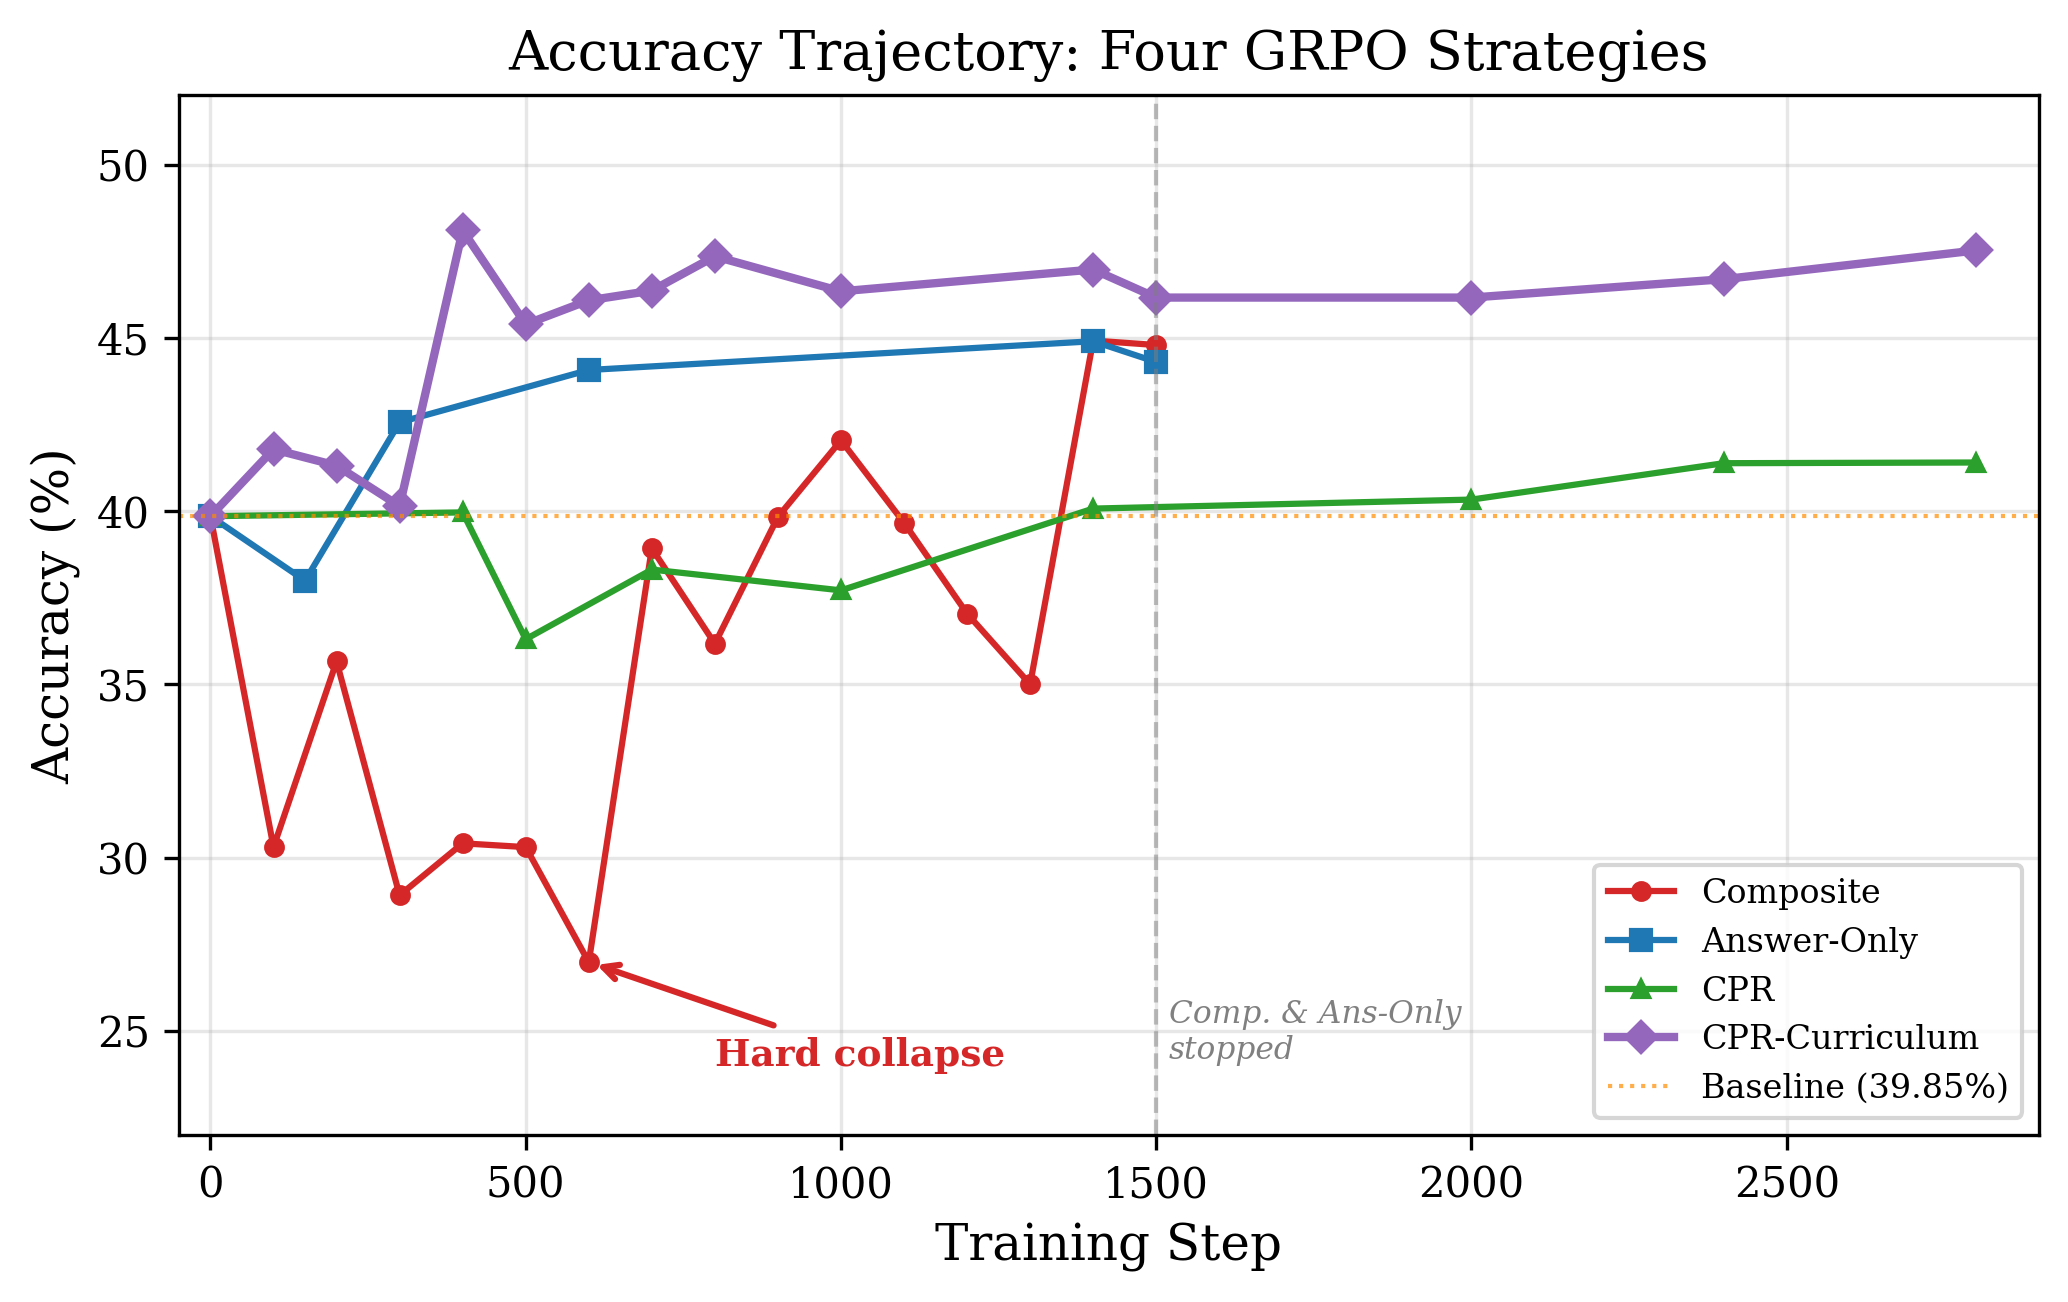
\includegraphics[width=\columnwidth]{figures/grpo_accuracy_trajectory.png}
\caption{\textbf{Accuracy alone is misleading.} Answer-Only reaches the highest accuracy (44.90\%) but its Match-F1 stays flat (see Figure~\ref{fig:f1_traj}), meaning reasoning never improves. Composite collapses at step 600. CPR sacrifices 3.5pp accuracy to gain +32\% in reasoning quality, the only strategy that improves both.}
\label{fig:acc_traj}
\end{figure}

\subsection{Cross-Strategy Analysis}

Table~\ref{tab:prec_recall} compares the precision/recall trade-off at each strategy's best checkpoint.

\begin{table}[t]
\centering
\caption{\textbf{Precision/Recall balance at best checkpoint.} Composite maximizes precision but collapses recall. CPR achieves the most balanced ratio.}
\label{tab:prec_recall}
\resizebox{\columnwidth}{!}{
\begin{tabular}{lccccc}
\toprule
& \textbf{Prec} & \textbf{Rec} & \textbf{P/R} & \textbf{Steps} & \textbf{F1 Std} \\
\midrule
Baseline    & 0.898 & 0.347 & 2.59$\times$ & 3.73 & $\pm$0.211 \\
Composite   & \best{0.983} & 0.284 & 3.46$\times$ & 3.00 & $\pm$0.132 \\
Answer-Only & 0.802 & 0.313 & 2.56$\times$ & 3.85 & $\pm$0.130 \\
\textbf{CPR}& \best{0.975} & \best{0.488} & \best{2.00$\times$} & \best{5.11} & $\pm$0.160 \\
\bottomrule
\end{tabular}
}
\end{table}

\noindent Composite pushes P/R to 3.46$\times$ (most imbalanced), generating only 3.00 steps on average. CPR achieves 2.00$\times$ (most balanced), generating 5.11 steps and covering 41\% more reference steps than baseline. Figure~\ref{fig:prec_rec_bars} visualizes this trade-off.

\begin{figure}[t]
\centering
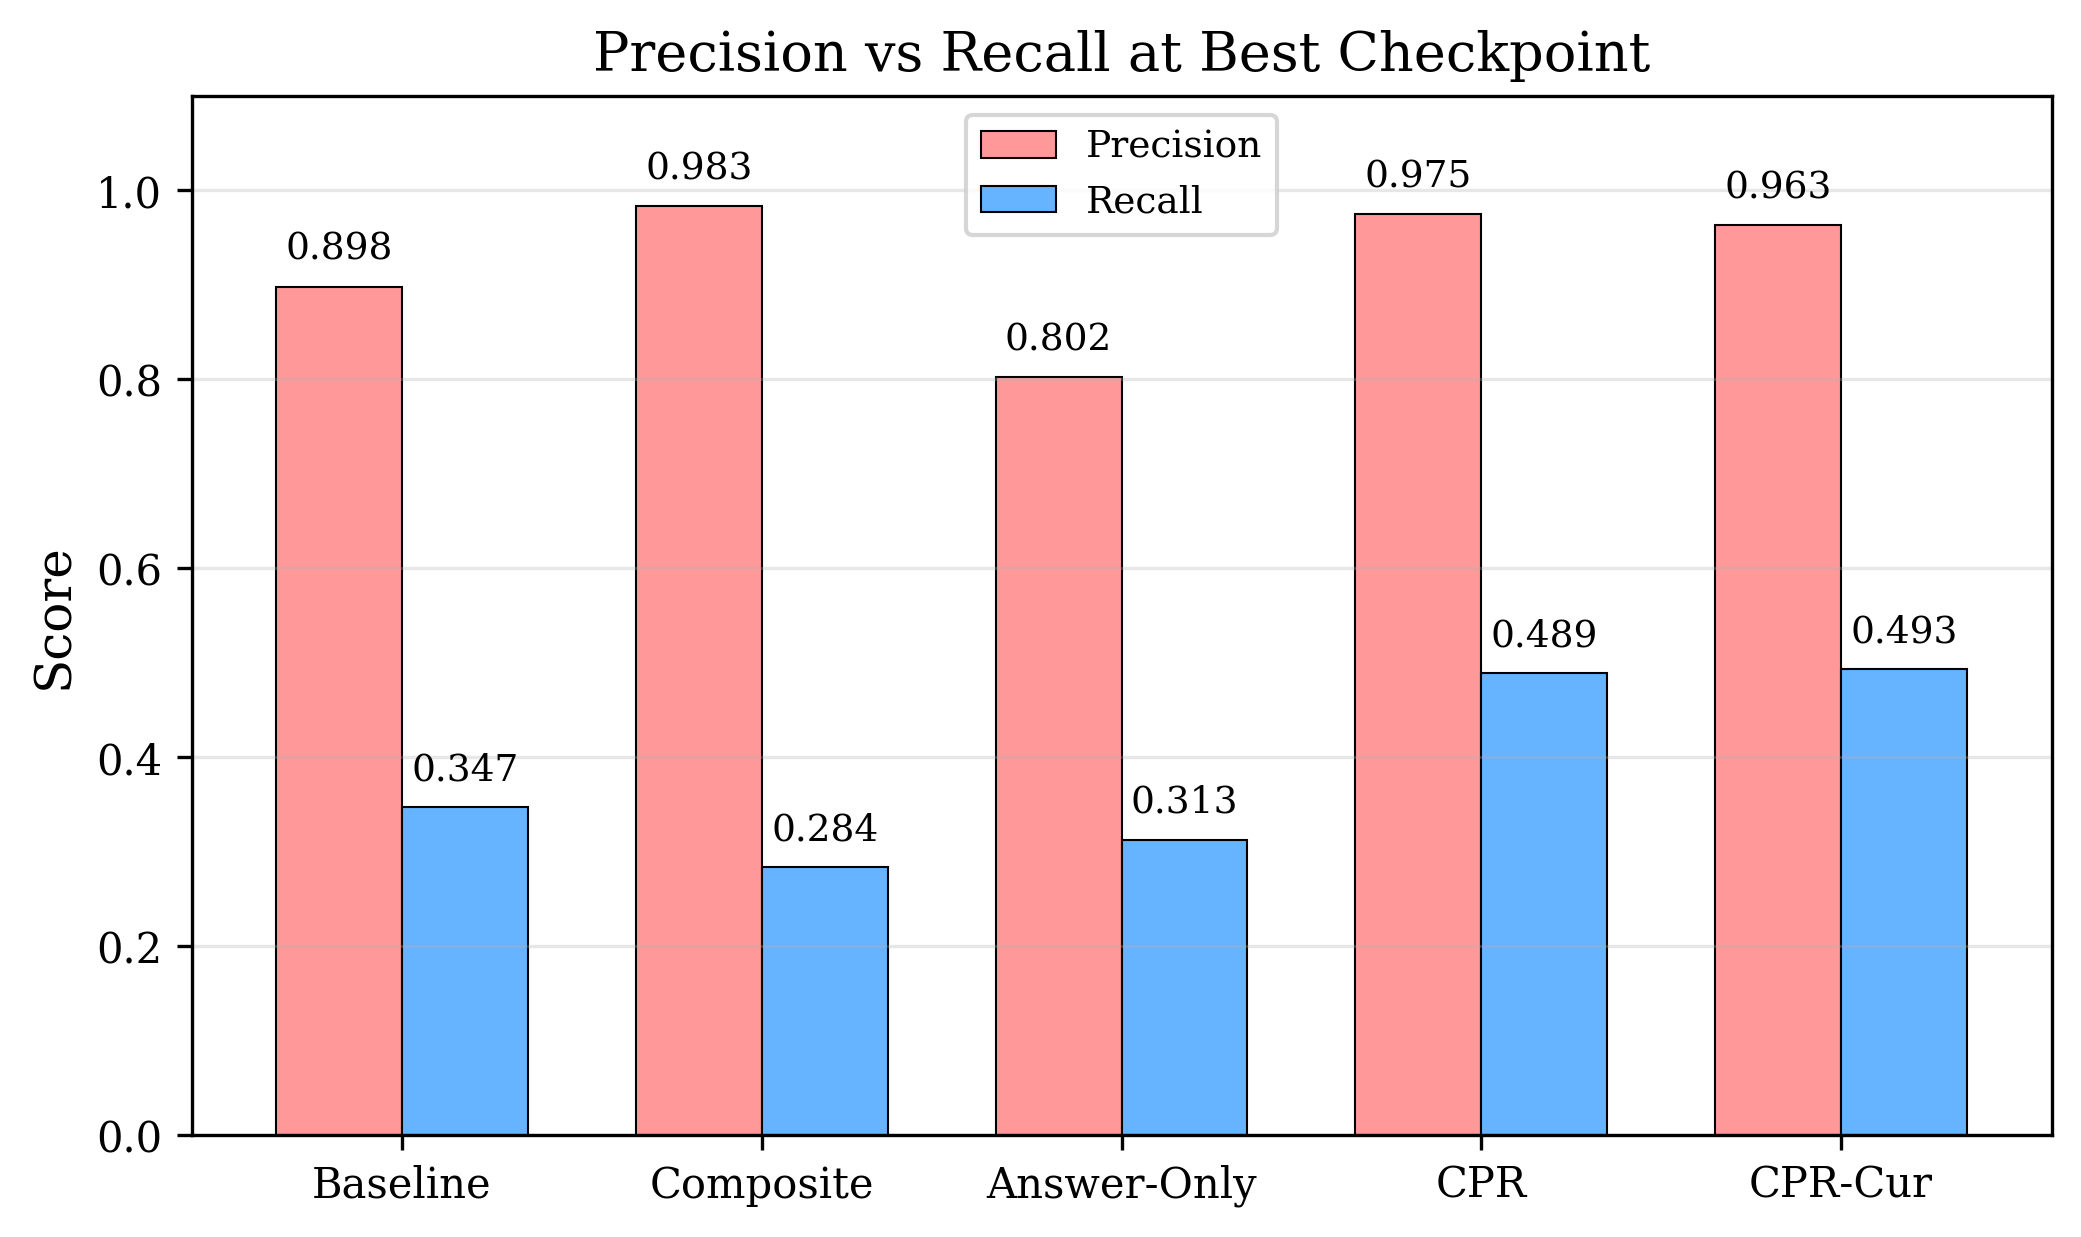
\includegraphics[width=\columnwidth]{figures/grpo_precision_recall_bars.png}
\caption{\textbf{Precision vs Recall at best checkpoint.} Composite maximizes precision (0.983) at the cost of recall (0.284). CPR achieves the highest recall (0.488) while maintaining near-identical precision (0.975), yielding the most balanced performance.}
\label{fig:prec_rec_bars}
\end{figure}

%%%%%%%%%%%%%%%%%%%%%%%%%%%%%%%%%%%%%%%%%%%%%%%%%%%%%%%%%%%%%%%%%%%%%%%%%%%%
\section{Responses to Reviewer GRPO Questions}
\label{sec:responses}
%%%%%%%%%%%%%%%%%%%%%%%%%%%%%%%%%%%%%%%%%%%%%%%%%%%%%%%%%%%%%%%%%%%%%%%%%%%%

\subsection{Reviewer Aho6}

\noindent\textbf{Q: ``GRPO surprisingly lowers Match-F1. I would expect it to increase monotonously.''}

Table~\ref{tab:headline} explains why: the original composite reward let accuracy dominate. Answer-Only reaches the same accuracy (44.90 vs 44.92\%) \textit{without any reasoning reward}, proving the accuracy component alone drives that gain. When reasoning is properly incentivized via CPR, Match-F1 \textit{does} increase: 0.480$\to$0.633 (+32\%), with monotonic improvement from step 700 to 2400 (Table~\ref{tab:cpr}).

\noindent\textbf{Q: ``The explanations are not convincing: references reflect ideal reasoning / shortcuts / semantic similarity.''}

We agree the original explanations were insufficient. The real cause is \textbf{reward imbalance}: in an additive composite $R = R_{\text{acc}} + R_{\text{reason}}$, the accuracy gradient is stronger and more consistent, dominating the reasoning signal. CPR solves this with multiplicative coupling: reasoning reward is \textit{gated} by answer correctness ($\times$0.3 penalty when wrong), preventing the model from optimizing accuracy at the expense of reasoning.

\noindent\textbf{Q: ``Compare GRPO with supervision from final answers only.''}

Done. Table~\ref{tab:answeronly} shows the full Answer-Only trajectory. Key result: Match-F1 stays flat (0.41 to 0.44) across all checkpoints, proving \textbf{reasoning does not improve without explicit reasoning reward}. This is the strongest evidence that Match-F1 captures genuine reasoning behavior, not a byproduct of accuracy training.

\noindent\textbf{Q: ``Why accuracy drops below baseline when accuracy is the reward'' (final justification).}

In Composite training, the mode collapse at step 600 (acc 26.98\%) occurs because format and reasoning rewards create conflicting gradients that temporarily destabilize accuracy. Answer-Only avoids this because it has only two aligned objectives (format + accuracy). CPR avoids it through PCGrad, which projects conflicting gradients to prevent destructive interference.

\noindent\textbf{Q: ``23.7\% Wrong+Sound cases not analyzed.''}

We analyzed 751 cases where F1~$\geq$~0.85 with wrong answers. Three root causes: \textbf{(1)~Error propagation:} sound reasoning chain with a single arithmetic error that invalidates the final answer. \textbf{(2)~MCQ extraction:} correct concept described in steps but wrong option letter selected (formatting issue). \textbf{(3)~Perception gap:} reasoning is logically sound given perceived elements, but initial visual perception was incorrect. This validates CRYSTAL's diagnostic value: it reveals \textit{where} failures occur (perception vs reasoning vs extraction).

\noindent\textbf{Q: ``No actionable insights for VLLM development.''}

Five recommendations from our expanded experiments: \textbf{(1)}~Separate perception from reasoning training (23.7\% of errors are perception, not reasoning). \textbf{(2)}~Target 7 to 10 reasoning steps (peak accuracy range; longer chains propagate errors). \textbf{(3)}~Use multiplicative rewards, not additive (prevents mode collapse). \textbf{(4)}~Focus training on recall, not precision (all models already achieve precision~$>$0.70). \textbf{(5)}~Enforce output format \textit{before} reasoning training (GRPO reduces refusals from 9.0\% to 1.3\%).

\subsection{Reviewer xNF6}

\noindent\textbf{Q: ``GRPO results need more discussion.''}

Tables~\ref{tab:composite}--\ref{tab:cpr} provide the full trajectories for three strategies with phase-by-phase analysis. The three-way comparison (Table~\ref{tab:headline}) directly demonstrates that step-level rewards produce measurably different reasoning behavior than answer-only training.

\subsection{Reviewer G1hH}

\noindent\textbf{Q: ``GRPO on Qwen2.5-VL, not a native reasoning model.''}

This is intentional: using a non-reasoning base model \textbf{isolates GRPO's effect}. If we used Qwen3-VL (which already has reasoning training), improvements would be confounded with pre-existing reasoning capabilities. The fact that CPR transforms a non-reasoning 3B model into one that generates 37\% more steps with 41\% higher recall demonstrates the training signal's effectiveness on a clean baseline.

\noindent\textbf{Q: ``Compare (your method + Qwen3-VL-instruct) vs (Qwen3-VL-thinking).''}

This is a valuable suggestion we acknowledge for future work. All our current GRPO experiments use Qwen2.5-VL-3B-Instruct as the base model. Figure~\ref{fig:cpr_dynamics} shows how CPR's self-correcting mechanism operates on this base, with accuracy and F1 co-evolving through distinct training phases.

\begin{figure}[t]
\centering
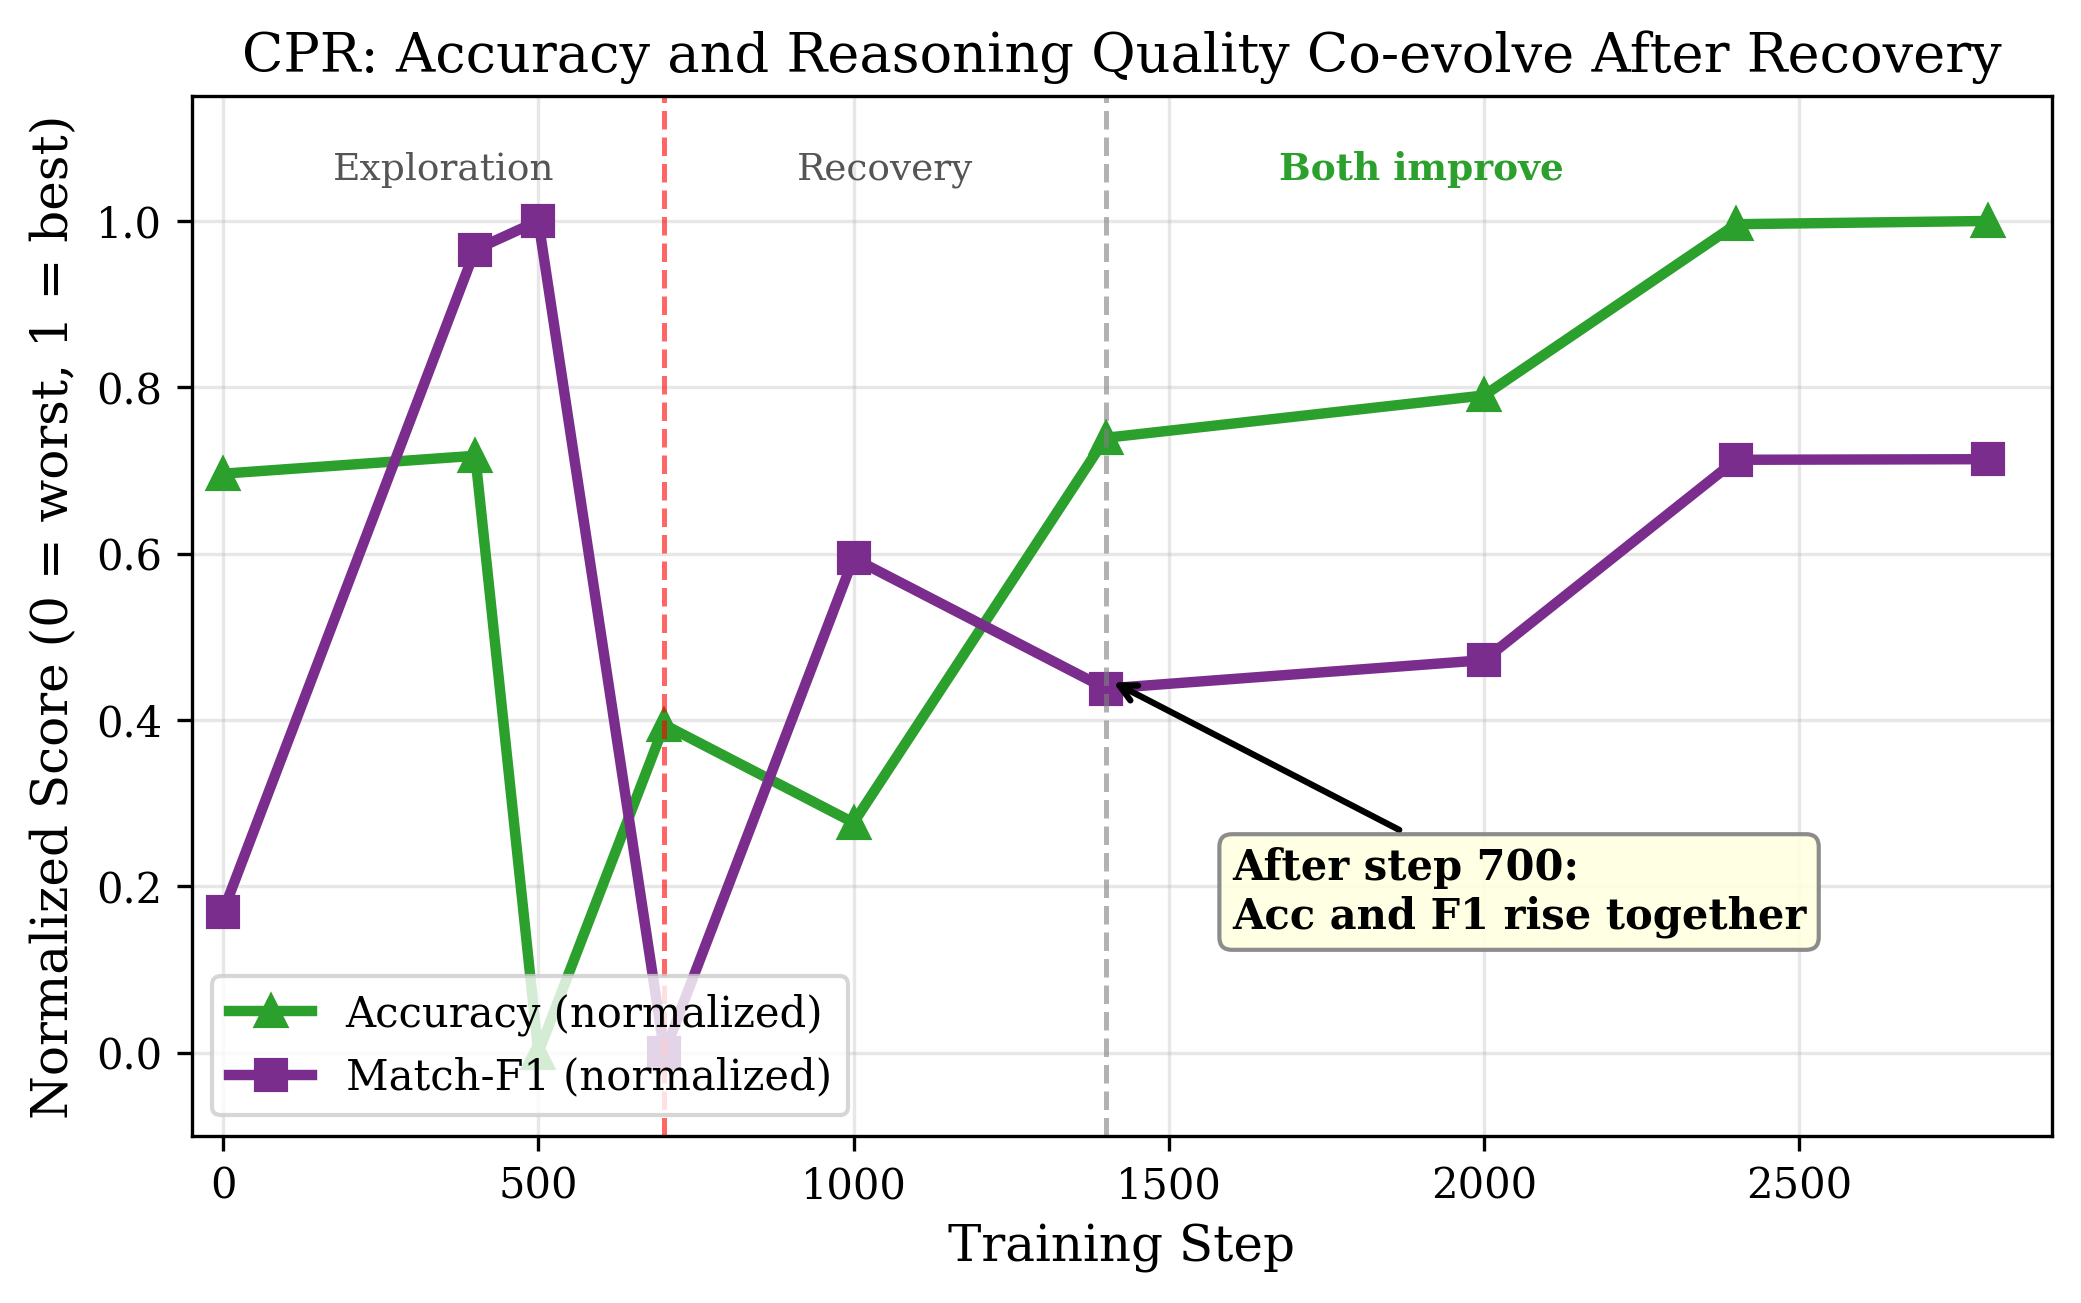
\includegraphics[width=\columnwidth]{figures/grpo_cpr_dynamics.png}
\caption{\textbf{CPR: accuracy and reasoning co-evolve.} Both metrics are normalized (0 = worst, 1 = best) for direct comparison. After a brief dip at step 700, accuracy and Match-F1 rise together through step 2400. This co-evolution is unique to CPR: Composite shows divergence (high accuracy, low F1) and Answer-Only shows stagnation (high accuracy, flat F1).}
\label{fig:cpr_dynamics}
\end{figure}

\subsection{Meta-Review}

\noindent\textbf{Q: ``GRPO decreased Match-F1, undermining the claim that the benchmark guides improvement.''}

We now show three results that collectively validate CRYSTAL as a training signal:
\begin{enumerate}[leftmargin=*,itemsep=1pt]
\item Answer-Only achieves the same accuracy as Composite but with flat F1, proving reasoning reward is necessary (and informative).
\item CPR achieves +32\% F1 over baseline with monotonic improvement from step 700 to 2400, proving Match-F1 \textit{can} increase with training when the reward structure is balanced.
\item The original F1 decrease was caused by reward imbalance (accuracy domination), not a flaw in the metric. CPR's multiplicative design prevents this.
\end{enumerate}

{\small
\bibliographystyle{ieeenat_fullname}
\begin{thebibliography}{9}
\bibitem{grpo} Z.~Shao et~al., ``DeepSeekMath: Pushing the limits of mathematical reasoning in open language models,'' \textit{arXiv:2402.03300}, 2024.
\bibitem{yu2020pcgrad} T.~Yu et~al., ``Gradient surgery for multi-task learning,'' \textit{NeurIPS}, 2020.
\end{thebibliography}
}

\end{document}
